\documentclass[12pt,twocolumn,letterpaper]{article}

%% Language and font encodings
\usepackage[english]{babel}
\usepackage[utf8x]{inputenc}
\usepackage[T1]{fontenc}

%% margins
\usepackage[margin=0.8in]{geometry}

%% captions
\usepackage[width=.45\textwidth]{caption}

%% Sets page size and margins
\usepackage[a4paper,top=3cm,bottom=2cm,left=3cm,right=3cm,marginparwidth=1.75cm]{geometry}

% make title page/contents one column (use the begin{strip}, end{strip}
\usepackage{cuted}

% citations
\usepackage[backend=biber,style=ieee,citestyle=numeric]{biblatex}

%% Useful packages
\usepackage{amsmath}
\usepackage{graphicx}
\usepackage[colorinlistoftodos]{todonotes}
\usepackage[colorlinks=true, allcolors=blue]{hyperref}
% \usepackage{natbib}
% \bibliographystyle{unsrt}
\usepackage{biblatex} %Imports biblatex package
\addbibresource{bibliography.bib} %Import the bibliography file
%% Title
\title{
		\usefont{OT1}{bch}{b}{n}

		\huge Franck-Hertz Experiment \\
}
\selectlanguage{english}
\usepackage{authblk}
\author[2]{Qingyuan Wu 1007001664, Regis Zhao 1007070660}


\begin{document}
\begin{strip} % strip prevents double column
\maketitle
\tableofcontents
\end{strip}


\section{Introduction}
In 1913, Bohr and Rutherford developed an atomic model that predicted that electrons can only occupy specific energy states surrounding the nucleus of an atom, instead of all regions close to the nucleus. This proposal was revolutionary in that it asserted energy is quantized \cite{bohr}. One year later, Franck and Hertz presented their now-famous Franck-Hertz experiment. They showed that incoming electrons lost their kinetic energies only in discrete amounts when they collided with mercury atoms. Below a certain threshold energy, the electrons merely bounced off of the mercury atoms without losing significant energy. However, at the threshold energy, the electron's velocity dropped to near zero. These experimental results were strong evidence supporting Bohr and Rutherford's quantum model of the atom. An electron can only transfer its kinetic energy to a mercury atom when the electron had enough energy to excite the one of mercury's valence electrons to the next energy level. Otherwise, no energy exchange occurs. Franck and Hertz won the 1925 Nobel prize for their findings \cite{franckhertzwiki}.

The purpose of this experiment is to imitate the original Franck-Hertz experiment and to compare our experimental findings with theirs.

\section{Materials \& Setup}
\begin{itemize}
    \setlength\itemsep{0em}
    \item Franck-Hertz tube with low pressure gas and some mercury vapour. The tube emits electrons through the cathode and accelerates them through a mesh grid \cite{Franck_theory}. The tube also had a collecting plate to measure the current of the collected electrons. A closeup of the tube is shown in Figure \ref{tube_picture}.
    \item Wires
    \item Mercury tube oven heater
    \item Electrometer
    \item Voltmeter
    \item \textit{FranckHertz.vi} data collection software
    \item Four DC voltage sources mounted on a panel:
    \begin{itemize}
        \item E1 is the filament supply,
        \item E2 is the screen grid voltage,
        \item E3 is the accelerating voltage,
        \item E4 is a fixed voltage to repel low energy electrons
    \end{itemize}
\end{itemize}

\begin{figure}
\centering

   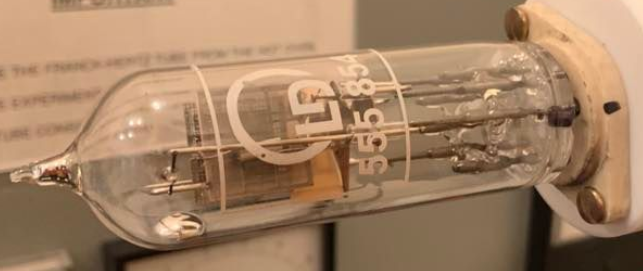
\includegraphics[width=0.45\textwidth]{figures/tube_picture.PNG}
%   \label{tube_picture} 

   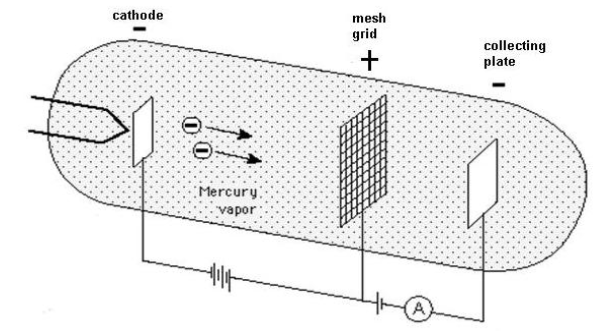
\includegraphics[width=0.45\textwidth]{figures/tube_schematic.PNG}
%   \label{tube_schematic}
\caption{Image of our tube (top) and a corresponding diagram (bottom).}
\label{tube_picture} % label must always be after caption
\end{figure}

\begin{figure}
  \centering
  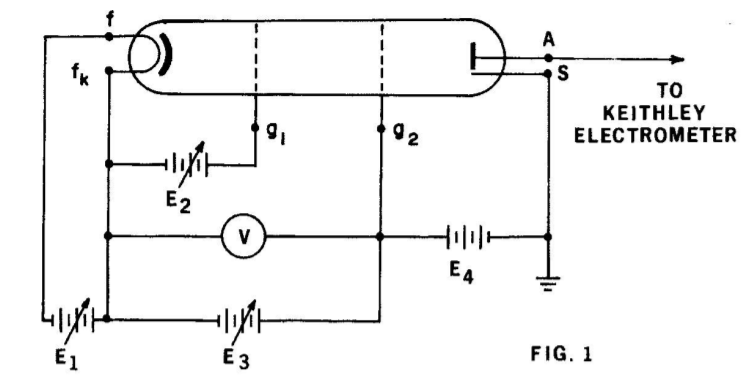
\includegraphics[width=0.45\textwidth]{figures/schematic.PNG}
  \caption{The wiring schematic of the Franck-Hertz tube.}
  \label{schematic}
\end{figure}

\begin{figure}
  \centering
  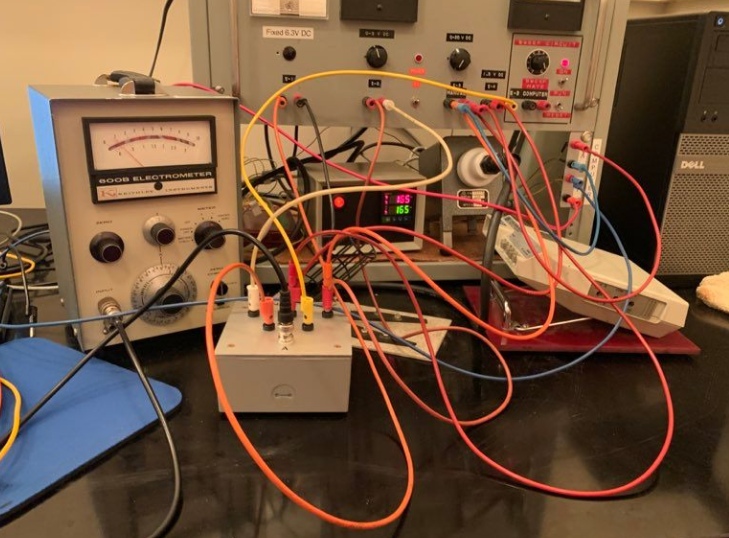
\includegraphics[width=0.45\textwidth]{figures/setup.PNG}
  \caption{Our experimental setup. The prism-shaped device on the table contained ports to the leads of the Franck-Hertz tube. E1-E4 voltage ports were mounted on the control panel.}
  \label{setup}
\end{figure}

\section{Methods}
The oven was turned on and, with the tube placed in it, was allowed to reach $170^\circ C$. Wires were used to connect the four voltage sources E1-E4 and leads to the Franck-Hertz tube, $f, f_k, g_1, g_2, s$. They were wired according to the schematic shown in Figure \ref{schematic}. Before collecting any data, we performed a manual voltage sweep to confirm that the setup was correct. The E3 voltage was connected to the \textit{Manual} panel ports and the E3 knob was slowly turned from $0V$ to $30V$. We observed were regularly spaced dips in the current reading, signifying that our setup was correct. E2 was adjusted between 1V and 2V to an optimal value for electrometer readings through trial and error. The data presented in this report used data collected for $E2 = 2V$. After the manual check, the E3 voltage and the electrometer were connected to the X and Y computer ports on the panel, respectively. To collect data for one sweep of the E3 voltage, the \textit{FranckHertz.vi} data collection software was used. The Sweep Circuit on the panel was switched to RESET, then RUN. The data for each trial was exported to a text file \cite{labmanual}.

\section{Analysis of Measured Data} \label{analysis}
The plots showing collected current vs. accelerating voltage data for the electrons are shown in this section. The experiment was conducted three times with varying values for $E2$. Ultimately, when $E2=2V$ the best results were observed as there were minimal outliers (sudden jumps or dips in the current values beyond the otherwise continuous and regularly repeating current vs. voltage pattern) in the data.

The most important measurement to take from the collected data was the voltage difference between consecutive peaks. Table \ref{peaks} shows the voltage value at each peak. $\Delta V$ is the difference in voltage between consecutive peaks. The average of the differences was $\Delta V_{ave} = 4.81 V$, not including peak 0. The first $\Delta V$ measurement was not included since the first peak was produced during the early stages of the experiment, before the current had stabilized and the relationship displayed a smooth pattern.

For comparison, the expected $\Delta V$ value, the one obtained by Franck and Hertz in their original experiment, was $4.90V$. The resulting expected wavelength of the emitted photon was $254 nm$ \cite{franckhertzedu}. 

\begin{table} % use table to add captions
\begin{center}
\begin{tabular}{|c c c|} 

 \hline
 Peak Number & Voltage (V) & $\Delta V$\\ [0.5ex] 
 \hline\hline
 0 & 6.73 & \\ 
 \hline
 1 & 11.13 &  4.40\\
 \hline
 2 & 15.91 &  4.78\\
 \hline
 3 & 20.66 & 4.75 \\
 \hline
 4 & 25.55 & 4.89 \\
 \hline

\end{tabular}
\caption{Table showing the voltage difference between current drops. All voltage peak readings had an uncertainty of $\pm 0.05V$, and the $\Delta V$ values have an uncertainty of $\pm 0.07V$. See Section \ref{error} for details. The peak numbers have no additional meaning beyond for labelling purposes}
\label{peaks}
\end{center}
\end{table}

\subsection{Sources of Error} \label{error}
All current and voltage data were generated by computer programs with high accuracy - the exported voltage data was accurate to six decimal places and the current data was accurate to five decimal places. Therefore, the measurement uncertainty for voltage was $\pm 5\cdot10^{-7}$, and the measurement uncertainty for current was $\pm 5\cdot10^{-6}$. Error bars were included in the plot but they were too small to be visible. Also, curve fitting was not appropriate in this context as the current vs. voltage plot contained over 1000 data points. The plot was not expected to follow a specific function or mathematical relationship. The main purpose of the graph was to show the current dips at specific voltage intervals. Therefore, the points were simply connected using smooth lines.

Since the process of locating local maxima was performed manually instead of using a computer program like the Python's scipy library's find\_peaks function, we estimate the error for the voltage readings for the peaks to have an uncertainty of $\pm 0.05 V$.

\begin{figure}
  \centering
  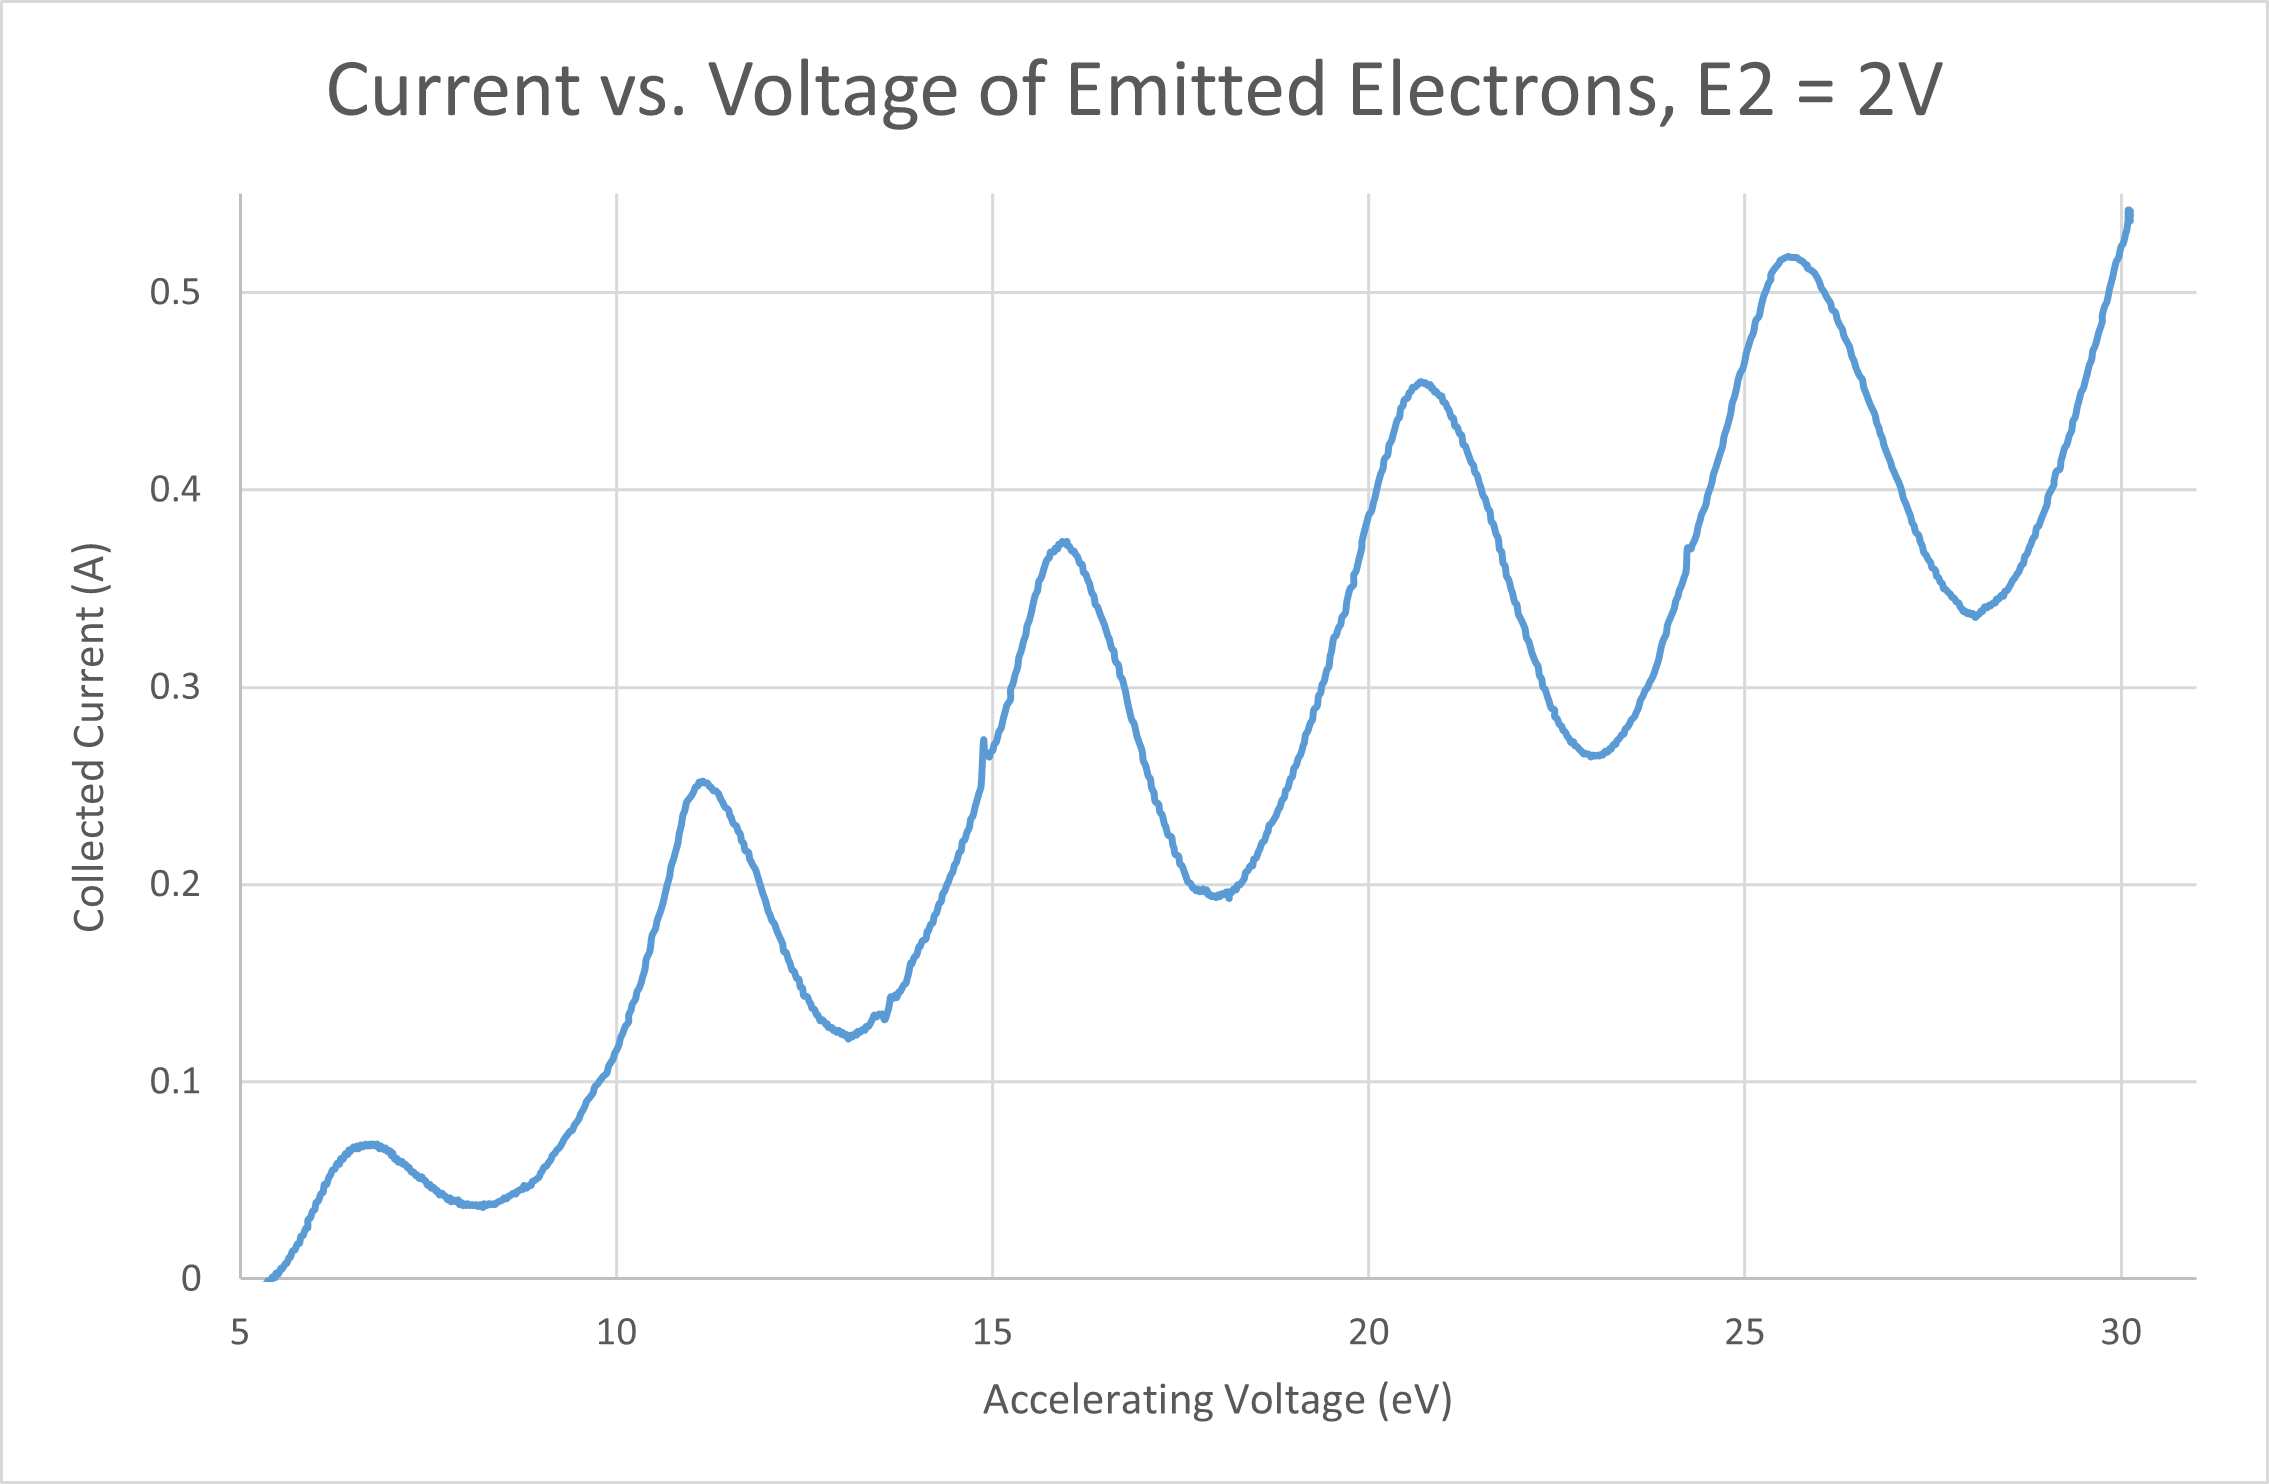
\includegraphics[width=0.5\textwidth]{figures/I vs A 2V.png}
  \caption{Current vs. Voltage with E3 = 2V.}
  \label{2V}
\end{figure}

The expected value for the voltage differences between current drops is $4.9 eV$ \cite{franckhertzedu}. The average value obtained from our experiment was $4.81eV \pm 0.07 eV$. The expected value lies just outside of our calculated value's uncertainty. Sources of error exist that affected the results we obtained. 
\\
Inaccuracies in the heating of the tube is one source of error. Both overheating and insufficient heating of the tube make it difficult to accurately identify the maxima and minima of the anode current; overheating significantly reduces emission current while insufficient heating significantly increases it \cite{labmanual}. Beyond the $\pm 0.5^\circ C$ instrumental uncertainty of the heater, it was extremely difficult to keep the temperature of the tube constant - even after setting the target temperature to $170^\circ C$, the tube's temperature would often overshoot or not reach the desired temperature. Tube temperature uncertainty was around $\pm 2^\circ C$. Another source of error is the difference in results due to varying screen grid voltage, E2. Inaccuracies in the calibration and sensitivity of the electrometer used to measure the anode current is another potential source of error.

\subsection{Calculating Uncertainties} \label{uncertainties}
Here, we find the uncertainty propagation for $\Delta V$. We use the propagation formula for addition and subtraction, $\delta (\Delta V) = \sqrt{\delta V_1^2 + \delta V_2^2}$, where $\delta$ represents the uncertainty of a variable.

\begin{align*}
    \delta (\Delta V) &= \sqrt{\delta V_1^2 + \delta V_2^2}\\
    \delta (\Delta V) &= \sqrt{0.05^2 + 0.05^2}\\
    \delta (\Delta V) &= 0.07 eV
\end{align*}

We calculate the uncertainty associated with the photon wavelength calculation. The formula for the wavelength of the photon $\lambda = hc/E$, which is discussed in more detail in Section \ref{q2}, will have uncertainties due to the propagation of the uncertainty associated with the energy of the photon, $E$. Note that $h$ and $c$ are constants, so they do not have uncertainties. Using the error propagation formula:
\begin{align*}
    \delta \lambda &= \lambda \sqrt{\frac{(\delta E)^2}{E^2}}\\
    \delta \lambda &= 258nm \sqrt{\frac{0.07^2}{4.81^2}}\\
    \delta \lambda &= 4nm
\end{align*}

We calculate the uncertainty of the wavelength to be $4nm$.
\section{Discussion}
\subsection{Amount of Energy Transferred from an Electron to a Mercury atom}

In an inelastic collision, all kinetic energy of the electron is transferred to the mercury atom. The amount of energy transferred from the electron to the mercury atom was $4.81 eV$ according to experimental results. As explained in Section \ref{analysis}, this value corresponds to the voltage difference between consecutive peaks in the current vs. accelerating voltage plot shown in Section \ref{2V}.

\subsection{Wavelength Associated with Photons Emitted by Mercury Atoms during Decay from the First Excited State to the Ground State} \label{q2}

Mercury atoms were measured to lose $4.81 eV$ when decaying from their first excited state to ground state, which is emitted as a photon. Therefore, $E_{photon}=4.81eV$. Using this fact along with the Planck-Einstein equation $E=hf$ and the wave speed equation $c=\lambda f$, where $h=4.136\cdot10^{-15}eVs$ is Planck's constant, $c=3.0\cdot10^8m/s$ is the speed of light, $f$ is the frequency, and $\lambda$ is the wavelength, we can find the wavelength of the excited photons.
\begin{align*}
    E_{photon} = hf &\hspace{0.5cm}\&\hspace{0.5cm}
    c = \lambda f\\
    \implies
    \lambda &= \frac{hc}{E_{photon}}\\
    \lambda &= \frac{(4.136\cdot10^{-15} eVs)(3.0\cdot10^8 m/s)}{4.81eV}\\
    \lambda &= 258 nm \pm 4 nm
\end{align*}

The uncertainty associated with the wavelength was due to error propagation from the $E_{photon}$ uncertainty. Details on this can be found in Section  \ref{uncertainties}.

\subsection{Why was Vaporized Mercury used instead of Hydrogen Gas?}
The Franck-Hertz experiment is ideally conducted with monoatomic gases (such as the noble gases) since if molecular gases are used, it is likely that the electrons will jump to molecular energy levels, differing from those of an atom itself \cite{modernphysics}. Therefore, hydrogen gas, $H_2$, is not a suitable gas to use due to its diatomic nature. Contrarily, vaporized mercury is a monoatomic gas, making it a more ideal gas to use for the Franck-Hertz experiment.

\subsection{Why are the Dips from the Current vs. Accelerating Voltage Graph not Sharp Sawtooth Patterns? How did this Affect your Results?}
In ideal conditions, the dips are expected to exhibit sharp sawtooth patterns, implying that \textit{all} electrons accelerated through the tube lose 4.9eV of energy once a sufficient voltage is applied. But in reality, not all electrons collide with mercury atoms, the collisions do not all occur simultaneously, and the process of settling to a steady probability of number of collisions is not an instantaneous one. Therefore we see a more gradual drop in the measured anode current from the experiment. This made it a bit more difficult to pinpoint the exact moment that the voltage began to drop which served as a source of uncertainty, therefore decreasing the accuracy of our results.

% The acquired current vs. accelerating voltage data did not have sharp sawtooth patterns because the rate of increase/decrease in current is continuous. Current and therefore energy cannot be transferred instantaneously. 

% A pretty good guide to formatting figures can be found at \url{https://en.wikibooks.org/wiki/LaTeX/Floats,_Figures_and_Captions#Figures}.
% \\

\section{Conclusions}
In this experiment, we demonstrated the discrete and quantized nature of mercury's energy levels. We found that electrons that bombarded mercury atoms in a cathode ray tube only transferred its energy for discrete values. These values were found to occur when the energy reached multiples of $4.81 eV \pm 0.07 eV$. Based on this value, the wavelength of the emitted photons were calculated to be $258 nm \pm 4 nm$. Although the expected value of $4.9 eV$ lies just outside of the uncertainty, the values are still very close and could be the result of other sources of error discussed earlier in the report that were unaccounted for. Regardless, the regularly-spaced dips in our plot of the anode current against the voltage is in agreement the original Franck-Hertz experiment and successfully confirms the quantum model of the atom. Furthermore, our calculated wavelength of the emitted photon agreed with the expected value of $254 nm$ within uncertainties. In the future, the quality of data collected could be improved by minimizing/eliminating the fluctuations in the temperature of the tube and ensuring the optimized calibration of the electrometer.

\section{Appendix}
\subsection{Raw Data}
More data were collected for $E2=1V$ and $E2 = 1.5V$. However, these were not used. Complete files of raw data can be accessed here: \url{https://github.com/qingyuan-wu/EngSci_Year2/tree/main/Franck-Hertz}.

\newpage
\section*{External Image Sources}
Figure \ref{tube_picture}: \\
\url{https://vlab.amrita.edu/?sub=1&brch=195&sim=355&cnt=1}
\\
Figure \ref{schematic}: \\
\url{https://q.utoronto.ca/courses/240175/pages/experiment-list-includes-links-to-all-manuals?module_item_id=2765499}
\\

\section{References}
\printbibliography
\end{document}
